% Texto restaurado a partir do PDF entregue.
\section{Identifica\c{c}\~ao experimental do modelo FOPDT}
\label{sec:identificacao_fopdt}

Esta se\c{c}\~ao descreve o procedimento adotado para estimar os
par\^ametros $K$, $L$ e $\tau$ da malha de velocidade a partir de
respostas a degrau obtidas em bancada. Os ensaios foram conduzidos com o
firmware instrumentado para emitir amostras de posi\c{c}\~ao e velocidade
via USART e SWV, em formato CSV, a partir das rotinas de telemetria do
servi\c{c}o de movimento. Para cada combina\c{c}\~ao de eixo e
microstepping, foi aplicado um perfil de degrau de velocidade gerado
pelo DDA, e os sinais de refer\^encia e medi\c{c}\~ao foram registrados
para posterior processamento em Python.

O m\'etodo opera inteiramente no dom\'inio do tempo, em linha com as
abordagens cl\'assicas de identifica\c{c}\~ao por curva de rea\c{c}\~ao, e
mostrou-se robusto a n\'iveis moderados de ru\'ido.

\subsection{Pr\'e-processamento e s\'eries derivadas}

Considere amostras ordenadas por tempo contendo os campos
$(t, p, c)$, em que $p$ representa a contagem acumulada de pulsos do
atuador e $c$ a contagem acumulada do encoder. A partir de pares de
amostras, ou de uma janela deslizante de comprimento $N$, definem-se
\begin{equation}
    \Delta t_k = t_k - t_{k-N+1},
    \qquad
    \Delta p_k = p_k - p_{k-N+1},
    \qquad
    \Delta c_k = c_k - c_{k-N+1},
\end{equation}
e as velocidades discretas
\begin{equation}
    v_{\text{cmd}}(k) = \frac{\Delta p_k}{\Delta t_k},
    \qquad
    v_{\text{enc}}(k) = \frac{\Delta c_k}{\Delta t_k}.
\end{equation}
Para reduzir o efeito de ru\'ido, utiliza-se tipicamente
$N \in [5,10]$. Pares com $\Delta t_k \le 0$ s\~ao descartados. O valor
de regime de cada s\'erie \'e obtido pela m\'edia dos \'ultimos 20\% da
janela temporal dispon\'ivel. Em outras palavras, a estima\c{c}\~ao usa a
parte final do ensaio como aproxima\c{c}\~ao do patamar em regime, o que
torna a extra\c{c}\~ao de ganho menos sens\'ivel a flutua\c{c}\~oes
instant\^aneas.

\subsection{Extra\c{c}\~ao de marcos temporais}

Define-se o in\'icio efetivo do degrau nos sinais de comando e de
medi\c{c}\~ao pelos primeiros cruzamentos de 5\% dos respectivos regimes:
\begin{equation}
    t^{\text{cmd}}_{5\%}
    =
    \inf \left\{ t : v_{\text{cmd}}(t) \ge 0{,}05 \bar{v}_{\text{cmd}} \right\},
    \qquad
    t^{\text{enc}}_{5\%}
    =
    \inf \left\{ t : v_{\text{enc}}(t) \ge 0{,}05 \bar{v}_{\text{enc}} \right\}.
\end{equation}
De forma an\'aloga, o instante $t_{63}$ \'e o primeiro cruzamento de
63,2\% do regime medido:
\begin{equation}
    t_{63}
    =
    \inf \left\{ t : v_{\text{enc}}(t) \ge 0{,}632 \bar{v}_{\text{enc}} \right\}.
\end{equation}

\subsection{Estimativas de $K$, $L$ e $\tau$}

O ganho est\'atico do modelo \'e calculado pela raz\~ao entre os regimes
do encoder e do comando:
\begin{equation}
    K = \frac{\bar{v}_{\text{enc}}}{\bar{v}_{\text{cmd}}}.
\end{equation}
O tempo morto \'e estimado por
\begin{equation}
    L = \max\left\{ 0, t^{\text{enc}}_{5\%} - t^{\text{cmd}}_{5\%} \right\},
\end{equation}
enquanto a constante de tempo decorre de
\begin{equation}
    \tau = t_{63} - L.
\end{equation}
Quando limita\c{c}\~oes de amostragem imp\~oem baixa resolu\c{c}\~ao
temporal, adota-se como piso o menor intervalo temporal observado na
s\'erie crua. Isso evita estimativas nulas ou negativas de $L$ e $\tau$,
que seriam incompat\'iveis com o modelo FOPDT adotado.

\subsection{S\'intese PD e valida\c{c}\~ao}

Com os par\^ametros $(K,L,\tau)$, computam-se os ganhos $K_p$ e $K_d$
pelas regras de Ziegler--Nichols para curva de rea\c{c}\~ao, mantendo
$K_i = 0$ na malha de velocidade. Em seguida, os ganhos cont\'inuos s\~ao
escalonados para o formato inteiro utilizado no firmware, preservando a
mesma conven\c{c}\~ao adotada no controlador discreto executado no STM32.

A valida\c{c}\~ao consiste em aplicar as constantes ao modelo FOPDT
discretizado com $T_s = \SI{1}{\milli\second}$ e comparar a resposta
simulada com a resposta medida, observando sobre-eleva\c{c}\~ao, tempo de
subida e aus\^encia de satura\c{c}\~oes relevantes.

\subsection{Valida\c{c}\~ao gr\'afica do modelo}

Para documentar a ader\^encia do modelo, foram gerados gr\'aficos de
sobreposi\c{c}\~ao entre a velocidade medida pelo encoder e a resposta
te\'orica do FOPDT a um degrau. A resposta empregada decorre da solu\c{c}\~ao
anal\'itica do sistema de primeira ordem com atraso:
\begin{equation}
    y(t) =
    \begin{cases}
        0, & t < L, \\
        K U \left(1 - e^{-(t-L)/\tau}\right), & t \ge L,
    \end{cases}
\end{equation}
em que a amplitude $U$ \'e tomada como a velocidade de comando em regime.
As Figuras~\ref{fig:fopdt-x}, \ref{fig:fopdt-y} e \ref{fig:fopdt-z}
mostram a compara\c{c}\~ao para os eixos X, Y e Z nos tr\^es n\'iveis de
microstepping avaliados.

\begin{figure}[H]
    \centering
    \begin{subfigure}{0.32\textwidth}
        \centering
        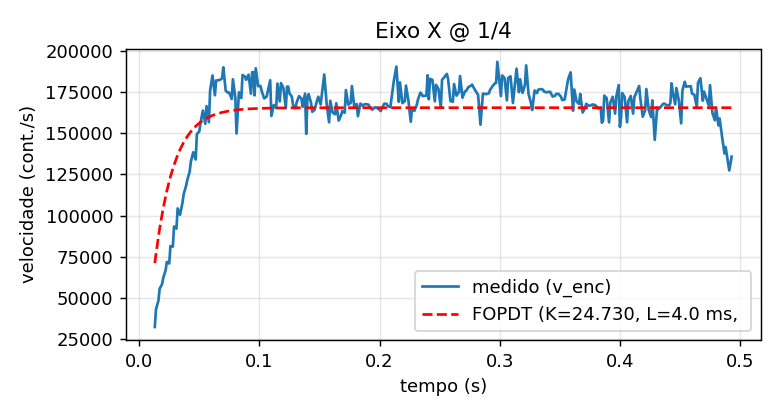
\includegraphics[width=\linewidth]{figures/pdf_recovered/fopdt_x_1_4.png}
        \caption{Eixo X @ 1/4.}
    \end{subfigure}
    \hfill
    \begin{subfigure}{0.32\textwidth}
        \centering
        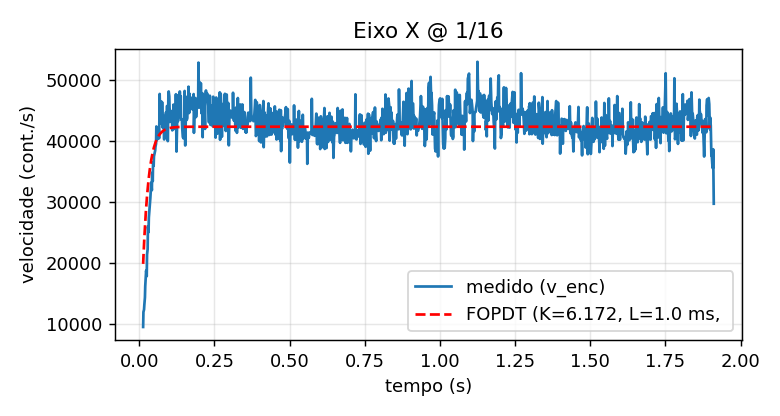
\includegraphics[width=\linewidth]{figures/pdf_recovered/fopdt_x_1_16.png}
        \caption{Eixo X @ 1/16.}
    \end{subfigure}
    \hfill
    \begin{subfigure}{0.32\textwidth}
        \centering
        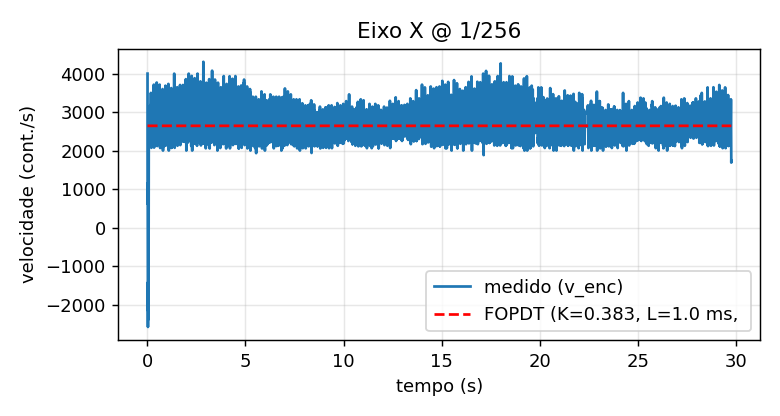
\includegraphics[width=\linewidth]{figures/pdf_recovered/fopdt_x_1_256.png}
        \caption{Eixo X @ 1/256.}
    \end{subfigure}
    \caption{Sobreposi\c{c}\~ao entre velocidade medida e resposta FOPDT para o eixo X.}
    \label{fig:fopdt-x}
\end{figure}

\begin{figure}[H]
    \centering
    \begin{subfigure}{0.32\textwidth}
        \centering
        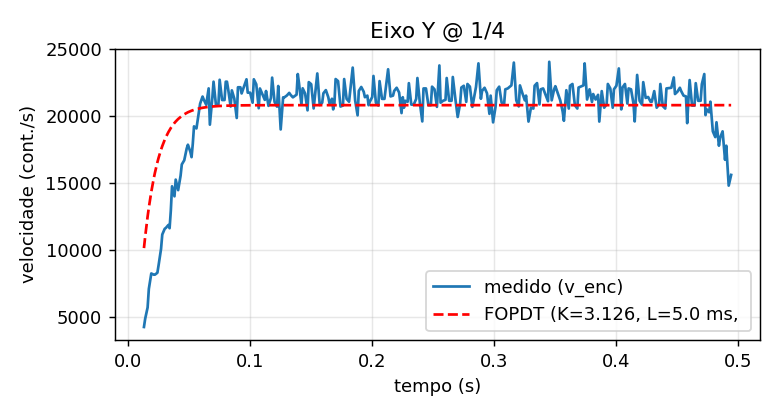
\includegraphics[width=\linewidth]{figures/pdf_recovered/fopdt_y_1_4.png}
        \caption{Eixo Y @ 1/4.}
    \end{subfigure}
    \hfill
    \begin{subfigure}{0.32\textwidth}
        \centering
        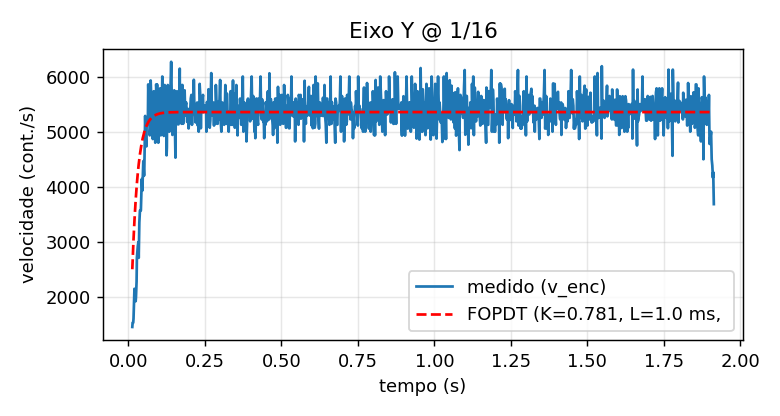
\includegraphics[width=\linewidth]{figures/pdf_recovered/fopdt_y_1_16.png}
        \caption{Eixo Y @ 1/16.}
    \end{subfigure}
    \hfill
    \begin{subfigure}{0.32\textwidth}
        \centering
        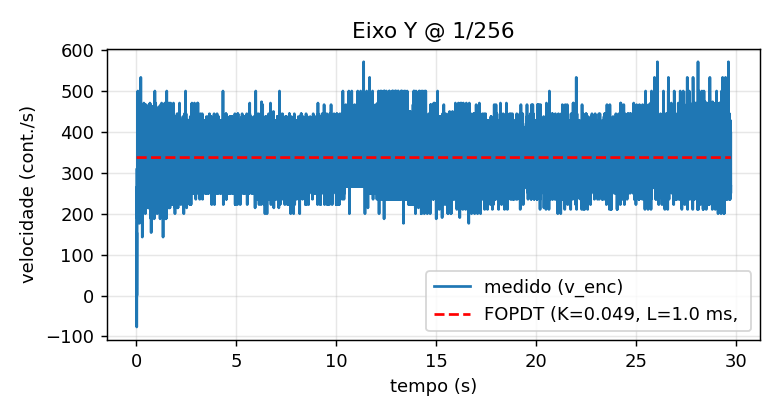
\includegraphics[width=\linewidth]{figures/pdf_recovered/fopdt_y_1_256.png}
        \caption{Eixo Y @ 1/256.}
    \end{subfigure}
    \caption{Sobreposi\c{c}\~ao entre velocidade medida e resposta FOPDT para o eixo Y.}
    \label{fig:fopdt-y}
\end{figure}

\begin{figure}[H]
    \centering
    \begin{subfigure}{0.32\textwidth}
        \centering
        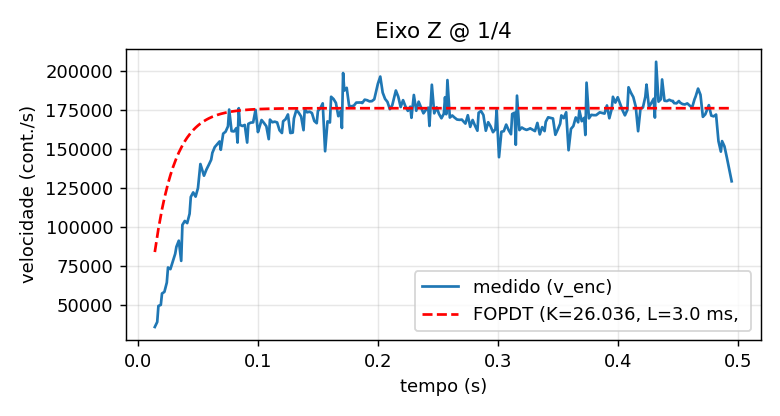
\includegraphics[width=\linewidth]{figures/pdf_recovered/fopdt_z_1_4.png}
        \caption{Eixo Z @ 1/4.}
    \end{subfigure}
    \hfill
    \begin{subfigure}{0.32\textwidth}
        \centering
        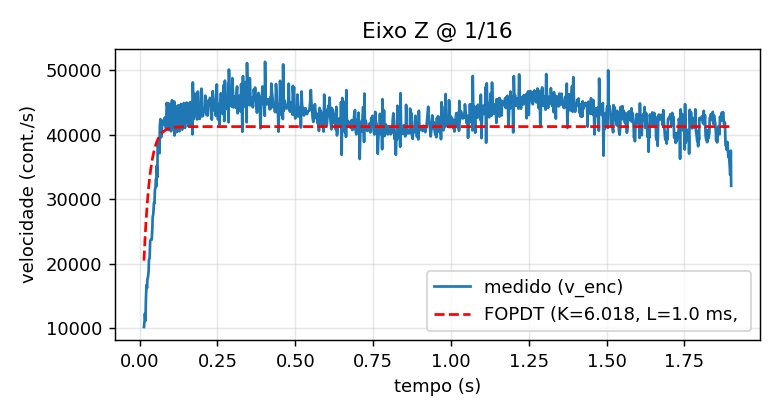
\includegraphics[width=\linewidth]{figures/pdf_recovered/fopdt_z_1_16.png}
        \caption{Eixo Z @ 1/16.}
    \end{subfigure}
    \hfill
    \begin{subfigure}{0.32\textwidth}
        \centering
        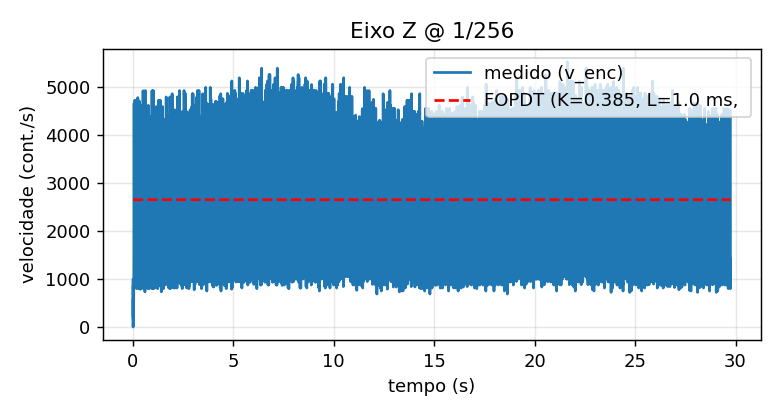
\includegraphics[width=\linewidth]{figures/pdf_recovered/fopdt_z_1_256.png}
        \caption{Eixo Z @ 1/256.}
    \end{subfigure}
    \caption{Sobreposi\c{c}\~ao entre velocidade medida e resposta FOPDT para o eixo Z.}
    \label{fig:fopdt-z}
\end{figure}

Observa-se que os microsteppings elevados, especialmente 1/256,
apresentam tempos caracter\'isticos menores e resposta mais ruidosa em
fun\c{c}\~ao da menor varia\c{c}\~ao incremental de velocidade. J\'a em
1/4, o ganho efetivo tende a ser maior e o atraso aparente cresce em
alguns eixos. As discrep\^ancias residuais s\~ao compat\'iveis com ru\'ido
de medi\c{c}\~ao, quantiza\c{c}\~ao temporal, atrito e pequenas n\~ao
linearidades mec\^anicas, mas a forma global da resposta permanece bem
representada pelo modelo FOPDT.
